%
%===============>>  ГРУППА 8-2 МОДУЛЬ 5  <<=============
%
\setmodule{5}

%BEGIN_FOLD % ====>>_____ Занятие 1 _____<<====
\begin{class}[number=1]
	\begin{listofex}
		\item Диагонали прямоугольника равны \( 8 \) и пересекаются
		под углом в \( 60\degree \).
		Найдите меньшую сторону прямоугольника.
		\item Угол при вершине \( A \) ромба \( ABCD \) равен \( 20\degree \). Точки \( M \) и \( N \) --- основания перпендикуляров, опущенных из вершины \( B \) на стороны \( AD \) и \( CD \).
		Найдите углы треугольника \( BMN \).
		\item Квадрат вписан в равнобедренный прямоугольный
		треугольник, причем одна вершина квадрата расположена на
		гипотенузе, противоположная ей вершина совпадает с вершиной
		прямого угла треугольника, а остальные лежат на катетах.
		Найдите сторону квадрата, если катет треугольника равен \( 12 \).
		\item На сторонах \( AB \) и \( CD \) прямоугольника \( ABCD \)
		взяты точки \( K \) и \( M \) так, что \( AKCM \) является ромбом.
		Диагональ \( AC \) составляет со стороной \( AB \) угол \( 30\degree \). Найдите сторону ромба, если наибольшая сторона прямоугольника \( ABCD \) равна \( 3 \).
		\item Докажите, что концы двух различных диаметров
		окружности являются вершинами прямоугольника.
		\item Через середину диагонали KM прямоугольника
		\( KLMN \) перпендикулярно этой диагонали проведена прямая,
		пересекающая стороны \( KL \) и \( MN \) в точках \( A \) и \( B \)
		соответственно. Известно, что \( AB = BM = 6 \).
		Найдите большую сторону прямоугольника.
		\item Окружность, построенная на стороне \( AD \)
		параллелограмма \( ABCD \) как на диаметре, проходит через вершину \( B \) и
		середину стороны \( BC \). Найдите углы параллелограмма.
		\item Решить уравнение:\quad\( (x-17)^2-7(x-17)+10=0 \)
	\end{listofex}
\end{class}
%END_FOLD

%BEGIN_FOLD % ====>>_____ Занятие 2 _____<<====
\begin{class}[number=2]
	\begin{listofex}
		\item Занятие 2
	\end{listofex}
\end{class}
%END_FOLD

%BEGIN_FOLD % ====>>_ Домашняя работа 1 _<<====
\begin{homework}[number=1]
	\begin{listofex}
		\item Докажите, что если в параллелограмме диагонали перпендикулярны, то такой параллелограмм --- ромб.
		\item Найдите расстояние от центра ромба до его стороны, если острый его угол равен \( 30\degree \), а сторона равна \( 4 \).
		\item Угол при вершине \( A \) ромба \( ABCD \) равен \( 60\degree \). На сторонах \( AB \) и \( BC \) взяты соответственно точки \( M \) и \( N \), причем \( AMBN \). Докажите, что треугольник DMN равносторонний.
		\item Докажите, что если в четырехугольнике три угла равны \( 90\degree \), то такой четырехугольник --- прямоугольник.
		\item \exercise{947}
	\end{listofex}
\end{homework}
%END_FOLD

%BEGIN_FOLD % ====>>_____ Занятие 3 _____<<====
\begin{class}[number=3]
	\begin{listofex}
		\item Вершины одного параллелограмма по одной лежат на сторонах другого. Докажите, что их центры совпадают.
		\item У двух параллелограммов совпадает пара противоположных вершин. Докажите, что остальные четыре их вершины образуют новый параллелограмм.
		\item На двух соседних сторонах параллелограмма построили равносторонние треугольники, как показано на рисунке. Докажите, что треугольник \( ABC \) равносторонний.
		\begin{center}
			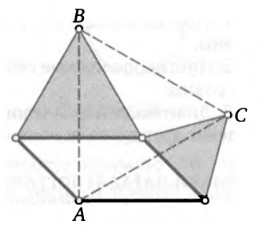
\includegraphics[align=t, width=0.35\linewidth]{\picpath/G82M5H1-1}
		\end{center}
		\item Вершины \( M \) и \( N \) равностороннего треугольника \( BMN \)
		лежат соответственно на сторонах \( AD \) и \( CD \) квадрата \( ABCD \).
		Докажите, что \( MN || AC \).
		\item Через центр квадрата проведены две взаимно
		перпендикулярные прямые. Докажите, что точки пересечения этих
		прямых со сторонами квадрата являются вершинами еще одного
		квадрата.
		\item Через произвольную точку внутри квадрата
		проведены две взаимно перпендикулярные прямые,
		каждая из которых пересекает две противоположные
		стороны квадрата. Докажите, что отрезки этих прямых,
		заключенные внутри квадрата, равны.
	\end{listofex}
\end{class}
%END_FOLD

%BEGIN_FOLD % ====>>_____ Занятие 4 _____<<====
\begin{class}[number=4]
	\begin{listofex}
		\item Биссектриса угла \( A \) параллелограмма \( ABCD \) пересекает сторону \( BC \) в точке \( K \). Найдите периметр параллелограмма, если \( BK  =  6 \), \( CK  =  10 \).
		\item Сумма двух противоположных углов параллелограмма в два раза больше суммы двух других углов. Найдите углы параллелограмма.
		\item На двух соседних сторонах параллелограмма построили равносторонние треугольники, как показано на рисунке. Докажите, что треугольник \( ABC \) равносторонний.
		\item Разность углов, прилежащих к одной стороне параллелограмма, равна \( 40\angle \). Найдите меньший угол параллелограмма. Ответ дайте в градусах.
		\begin{center}
			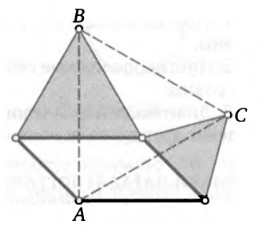
\includegraphics[align=t, width=0.35\linewidth]{\picpath/G82M5H1-1}
		\end{center}
		\item У двух параллелограммов совпадает пара противоположных вершин. Докажите, что остальные четыре их вершины образуют новый параллелограмм.
		\item Вершины \( M \) и \( N \) равностороннего треугольника \( BMN \)
		лежат соответственно на сторонах \( AD \) и \( CD \) квадрата \( ABCD \).
		Докажите, что \( MN || AC \).
		\item Через центр квадрата проведены две взаимно
		перпендикулярные прямые. Докажите, что точки пересечения этих
		прямых со сторонами квадрата являются вершинами еще одного
		квадрата.
	\end{listofex}
\end{class}
%END_FOLD

%BEGIN_FOLD % ====>>_ Домашняя работа 2 _<<====
\begin{homework}[number=1]
	\begin{listofex}
		\item Биссектриса внутреннего угла при вершине A и биссектриса внешнего угла при вершине \( C \) треугольника \( ABC \)
		пересекаются в точке \( M \). Найдите \( \angle BMC \), если \( \angle BAC = 40\degree \) и \( \angle ABC = 60\degree \).
		\item Докажите, что если в параллелограмме две смежные стороны равны, то такой параллелограмм --- ромб.
		\item Угол при вершине \( A \) ромба \( ABCD \) равен \( 20\degree \). Точки \( M \) и \( N \) --- основания перпендикуляров, опущенных из вершины \( B \) на стороны \( AD \) и \( CD \). Найдите углы треугольника \( BMN \).
		\item Докажите, что если в параллелограмме один из углов равен \( 90\degree \), то такой параллелограмм --- прямоугольник.
		\item Диагонали прямоугольника равны \( 8 \) и пересекаются под углом \( 60\degree \). Найдите меньшую сторону прямоугольника.
	\end{listofex}
\end{homework}
%END_FOLD

%BEGIN_FOLD % ====>>_____ Занятие 5 _____<<====
\begin{class}[number=5]
	\begin{listofex}
		\item Решить уравнения:
		\begin{tasks}(1)
			\task \( -3x^2+4x-7=-x^2+5x-(-1+2x^2) \)
			\task \( (x+2)^2+(x-3)^2=2x^2 \)
		\end{tasks}
		\item В треугольнике \( ABC \) высота \( CD=15 \), \( AB=22 \). Найдите площадь треугольника \( ABC \).
		\item В равнобедренном треугольнике \( ABC \, \angle B=30\degree \), \( AB=AC=8 \). Найдите площадь треугольника \( ABC \).
		\item В прямоугольном треугольнике \( ABC \, \angle C=90\degree\), \( AC=9 \), \( BC=4 \). Найдите площадь треугольника \( ABC \).
		\item Докажите, что площадь параллелограмма равна произведению стороны на опущенную на неё высоту.
		\item Площадь параллелограмма равна \( 36,3 \) дм\( ^2 \), высота --- \( \mfrac{4}{1}{3} \) дм. Найдите сторону параллелограмма, к которой проведена высота.
		\item Высота \( BE \) делит сторону \( AD \) параллелограмма \( ABCD \) на отрезки, равные \( 6 \) и \( 3 \). \( AB=8 \), \( \angle A=30\degree \). Найдите площадь параллелограмма.
		\item Периметр параллелограмма равен \( 40 \), меньшая сторона равна \( 4 \). Найдите площадь параллелограмма, если его острый угол равен \( 60\degree \).
		\item Площадь параллелограмма равна \( 40 \), а две его стороны равны \( 5 \) и \( 10 \). Найдите его высоты. В ответе укажите большую высоту.
		
	\end{listofex}
\end{class}
%END_FOLD

%BEGIN_FOLD % ====>>_____ Занятие 6 _____<<====
\begin{class}[number=6]
	\begin{listofex}
		\item Сколько понадобится краски, чтобы покрасить панно, которое имеет форму ромба с диагоналями \( 5 \) дм и \( 3,4 \) дм, если на \( 1 \) дм\( ^2 \) расходуется \( 2 \) г краски?
		\item В прямоугольнике диагонали пересекаются в точке \( O \). \( E \) --- середина стороны \( AB \), \( \angle BAC=50\degree \). Найдите \( \angle EOD \).
		\item Найти диагональ \( PF \) ромба \( KPRF \), если \( KR =4 \) см, \( S KPRF=28 \) cм\( ^2 \).
		\item Диагонали ромба относятся как \( 3:5 \), а их сумма равна \( 16 \) см. Найти площадь ромба.
		\item Найдите  площадь ромба  \( ABCD \), если \( AO = 4  \) см, \( BO = 2,5 \) см, где  \( O \) --- точка пересечения диагоналей ромба.
		\item На стороне \( AD \) параллелограмма \( ABCD \) взята точка \( E \) так, что \( AE = 4 \) см, \( ED = 5 \) см, \( BE = 12 \) см, \( BD = 13 \) см. Найдите площадь параллелограмма.
		\item В выпуклом четырехугольнике \( ABCD \) проведены диагонали. Известно, что площади треугольников \( ABD \), \( ACD \), \( BCD \) равны. Докажите, что данный четырехугольник является параллелограммом.
	\end{listofex}
\end{class}
%END_FOLD

%BEGIN_FOLD % ====>>_ Домашняя работа 3 _<<====
\begin{homework}[number=3]
	\begin{listofex}
		\item Решить уравнения:
		\begin{tasks}(2)
			\task \( x^2+7x-18=0 \)
			\task \( x^2+4=5x \)
			\task \( \dfrac{5}{4}x^2+7x+9=0 \)
			\task \( (x+10)^2=(5-x)^2 \)
		\end{tasks}
		 \item В параллелограмме \( ABCD \) \( AB=12 \), высоты \( DH \) и \( DE \) равны \( 5 \) и \( 10 \) соответственно. Найдите \( BC \).
		 \item Высота \( BE \) делит сторону \( AD \) параллелограмма \( ABCD \) на отрезки, равные \( 6 \) и \( 3 \). \( AB=8 \), \( \angle A=30\degree \). Найдите площадь параллелограмма.
	\end{listofex}
\end{homework}
%END_FOLD

%BEGIN_FOLD % ====>>_____ Занятие 7 _____<<====
\begin{class}[number=7]
	\title{Подготовка к проверочной}
	\begin{listofex}
		\item \( ABCD \) --- параллелограмм; \( P_{ABCD}=10 \) см; \( P_{ABD}=8 \)  см. Найти: \( BD \).
		\item \( ABCD \) --- параллелограмм; \( AK \) --- биссектриса \( \angle A \); \( BK:KC=2:1 \); \( P_{ABCD}=50 \) см. Найти: \( AB \); \( BC \); \( CD \); \( AD \).
		\item \( ABCD \) --- квадрат. \( AC=4 \), \( O \) --- точка пересечения диагоналей. Точку \( K \) взяли так, что \( OBKC \) тоже квадрат. Найдите сторону квадрата \( OBKC. \)
		\item Треугольник \( ABC \) --- равнобедренный, \( \angle A=90\degree \). В него вписан квадрат \( AB_1DC_1 \) так, что \( B_1 \) лежит на \( AB \) и \( C_1 \) на \( AC \); \( AB = 2 \) см. Найдите периметр квадрата \( AB_1DC_1  \).
		\item Чему равна площадь треугольника; параллелограмма; ромба?
		\item Периметр ромба равен \( 60 \), а один из его углов --- \( 30\degree \). Найдите площадь ромба.
		\item Площадь параллелограмма равна \( 32 \), а две его стороны равны \( 8 \) и \( 16 \). Найдите его высоты. В ответе укажите большую высоту.
		\item Решить уравнения:
		\begin{tasks}(2)
			\task \( x^2-x-6=0 \)
			\task \( 4x^2+4x+1=(x-2)^2 \)
			\task \( 3x^2+x-5=0 \)
		\end{tasks}
		\item \exercise{1473}
	\end{listofex}
\end{class}
%END_FOLD

%BEGIN_FOLD % ====>>_ Проверочная работа _<<====
\begin{exam}
	\begin{listofex}
		\item Периметр ромба равен \( 88 \), а один из его углов --- \( 30\degree \). Найдите площадь ромба.
		\item В параллелограмме \( ABCD \) \( AB=6 \), \( \angle A=30\degree \). Высота \( BE \) делит сторону \( AD \) на отрезки, равные \( 6 \) и \( 3 \). Найдите площадь параллелограмма.
		\item Одна из сторон параллелограмма в \( 3 \) раза меньше другой, а его периметр равен \( 72 \) см. Найдите стороны параллелограмма.
		\item Биссектриса угла \( D \) параллелограмма \( ABCD \) пересекает сторону \( BC \) в точке \( M \),\( BM:MC=4:3 \). Найдите периметр параллелограмма, если \( BC=28 \) см.
		\item Один из углов ромба равен \( 64\degree \). Найдите углы, которые образует сторона ромба с его диагоналями.
		\item Диагонали прямоугольника \( ABCD \) пересекаются в точке \( O \), \( CD=15 \) см, \( AC=20 \) см. Найдите периметр треугольника \( AOB \).
		\item Докажите, что биссектрисы односторонних углов параллелограмма --- перпендикулярны.
		\item Решите уравнения:
		\begin{tasks}(2)
			\task \( 6x^2+x-2=0 \)
			\task \( (3x+1)^2=(x+2)^2 \)
		\end{tasks}
		\item Упростите выражение: \quad \( \left( \dfrac{y^2-xy}{x^2+xy}-xy+y^2 \right)\cdot\dfrac{x}{x-y}+\dfrac{y}{x+y} \)
	\end{listofex}
\end{exam}
%END_FOLD
